\documentclass[conference]{IEEEtran}
\IEEEoverridecommandlockouts
% The preceding line is only needed to identify funding in the first footnote. If that is unneeded, please comment it out.
\usepackage{cite}
\usepackage{amsmath,amssymb,amsfonts}
\usepackage{algorithmic}
\usepackage{graphicx}
\usepackage{textcomp}
\usepackage{xcolor}
\def\BibTeX{{\rm B\kern-.05em{\sc i\kern-.025em b}\kern-.08em
    T\kern-.1667em\lower.7ex\hbox{E}\kern-.125emX}}
\begin{document}

\title{Detecting Stack Overflow In-line Codes by Language Model\\
}

\author{\IEEEauthorblockN{Yixing Luan}
\IEEEauthorblockA{\textit{Department of Computing Science} \\
\textit{University of Alberta}\\
Edmonton, Canada \\
yixing1@ualberta.ca}
\and
\IEEEauthorblockN{Shutong Li}
\IEEEauthorblockA{\textit{Department of Computing Science} \\
\textit{University of Alberta}\\
Edmonton, Canada \\
shutong@ualberta.ca}
\and
\IEEEauthorblockN{Rashed Rubby Riyadh}
\IEEEauthorblockA{\textit{Department of Computing Science} \\
\textit{University of Alberta}\\
Edmonton, Canada \\
riyadh@ualberta.ca}
\and
\IEEEauthorblockN{Alexander William Wong}
\IEEEauthorblockA{\textit{Department of Computing Science} \\
\textit{University of Alberta}\\
Edmonton, Canada \\
alex.wong@ualberta.ca}
\and
\IEEEauthorblockN{Grzegorz Kondrak}
\IEEEauthorblockA{\textit{Department of Computing Science} \\
\textit{University of Alberta}\\
Edmonton, Canada \\
gkondrak@ualberta.ca}
\and
\IEEEauthorblockN{Abram Hindle}
\IEEEauthorblockA{\textit{Department of Computing Science} \\
\textit{University of Alberta}\\
Edmonton, Canada \\
hindle1@ualberta.ca}
}

\maketitle

\begin{abstract}
 Stack Overflow is one of the most popular online discussion forums of programming problems. Usually, posts on Stack Overflow can be divided into two different kinds of blocks: text blocks and code blocks. In text blocks, users provide questions, answers and explanations in natural language text. In the code blocks, users provide actual codes or commands to provide the detailed situations or solutions. However, sometimes, users include simple codes or commands into text blocks as in-line codes. These in-line codes contain crucial information but are not distinguished from other natural language sentences in existing database. Therefore, when mining codes from  data, those in-line codes are often missed. This paper presents an approach to distinguish in-line codes in text blocks by using simple language models. To build the language model, we use code blocks extracted from SOTorrent, which is a torrent data obtained from Stack Overflow dump data. For the evaluation, due to the lack of labelled in-line code in Stack Overflow dataset, we also manually labelled extracted text data to create test dataset. We also expect this model can be used in other situations that developers want to extract codes from natural language text.
\end{abstract}

\begin{IEEEkeywords}
Stack Overflow, SOTorrent, language model
\end{IEEEkeywords}

\section{Introduction}
These days, many people are using Stack Overflow to discuss the programming problems. Because of its wide coverage of topics and the huge number of users, Stack Overflow is becoming more and more popular. Therefore, there is a lot of log data, which contains posts, comments, user information, and so on. In order to take an advantage of this large amount of data, Stack Overflow published an official Stack Overflow data dump\cite{b1}. Then, in order to deeply analyze the evolution of Stack Overflow posts, Stack Overflow torrent (SOTorrent) is published\cite{b2}\cite{b3}. In addition to all tables in Stack Overflow data dump, additional tables, which are extracted from Stack Overflow posts by combining them with external sources such as Google BigQuery and GitHub dataset, are included in SOTorrent. The 

In current situation, it is difficult to extract in-line codes, which are simple codes or commands included in natural language text, from these StackOverflow data dump or SOTorrent. In SOTorrent, text blocks and code blocks are separated, but short codes or commands in text blocks, which are in-line codes, are not clearly distinguished. However, it is usual that Stack Overflow users include in-line codes in text blocks, and these in-line code sometimes provide crucial information to solve programming problems. Therefore, it will be helpful for Stack Overflow users if in-line codes are easily detected. 

In order to detect in-line codes in text blocks, we use language models. Language models are widely used in natural language processing research and can be applied to various tasks such as text classification, language identification, and so on. So, if we treat codes as texts and train a language model with them, we can build the language model, which can distinguish in-line codes and natural language sentences. In addition, we also apply text classification model to this task to compare with simple language models.


\section{Methods}
In this section, we present the methods to detect in-line codes. First, we discuss how we extract training data and create test data. Then, we discuss the language models we used for our task.

\subsection{Data Mining and Preprocessing}
1.	training data

This paper uses two training sets for natural language and programming language respectively. We cannot use text with in-line code for training because there is no enough labelled inline code. The programming language data set is codes extracted from the latest version of code blocks in SOTorrent. 

2.	test data

To test the methods of this paper, we used three test sets, which are all negative test set, all positive test set and real situation test set.

The all negative test set and all positive test set are from Opensubtitle and code blocks. 

In order to test the performance of our method in real situation, this paper create a test case from Stack overflow, which contains 161 pure natural language sentences and 139 sentences with inline code. Compared with the OpenSubtitles, natural language sentences in this test case are related with computing science instead of movies or music. As a result, they have some words that are commonly seen in code but never appear in our training set of natural language, for example, NumPy. And this may cause false positive. For the text with inline code, the portion of natural language in sentences can affect the result, because they are similar to natural language in different degree. To sum up, this test case is harder for our method and will indicates the real performance of it.


\begin{figure*}[ptbh]
\begin{center}
  \centering
  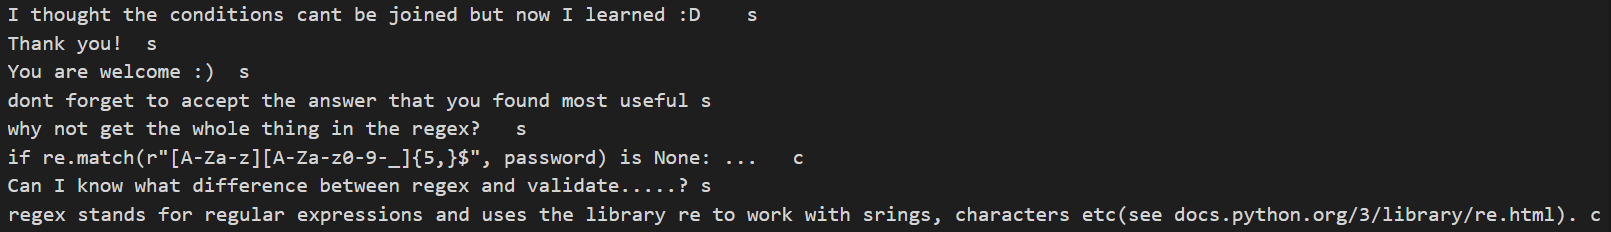
\includegraphics[width=16cm]{manualdata.png}
  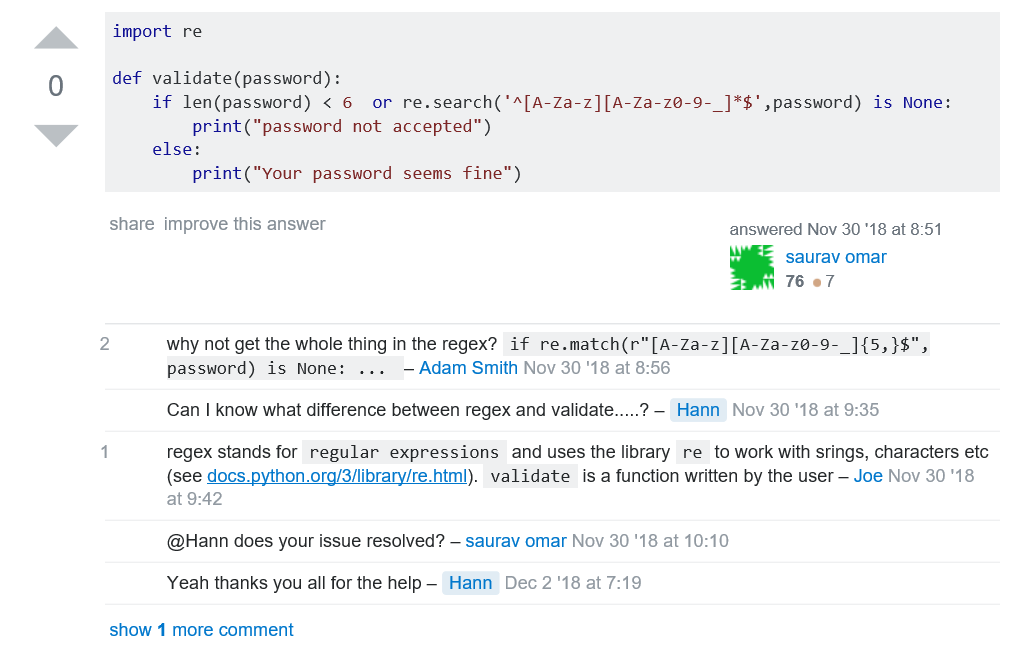
\includegraphics[width=16cm]{SOpage.png}
  \caption{The example of manually created test data and corresponding Stack Overflow page}
 \end{center}
\end{figure*}



\subsection{N-gram Language Models}
In order to distinguish in-line codes from natural language sentences, we treat the task as a binary classification problem. Therefore, our goal is to classify each sentence to whether it contains codes (in-line code) or not (natural language sentence). We build two n-gram language model and train each of them by using natural language text data and pure code data. Then, for each line, we compare the probabilities of both models to decide the class. 

N-gram language models are one of the simplest probabilistic language models and are widely used as a baseline. N-gram language models are based on a simple assumption that the probability of the current word only depends on the n-1 previous words. The number n determines how long we should consider for the current word. Usually, too small n makes the model too general to correctly predict the probability, and too large n makes it difficult to match n-grams because of many unseen sequences.

In order to build a effective n-gram language model, we have to use smoothing methods to prevent a zero probability. In our methods, we use a major smoothing method, linear interpolation smoothing. Linear interpolation does smoothing by taking the weighted sum of all estimated n-gram probabilities. To get the weight values, we used the deleted interpolation algorithm. 

We used natural language toolkit (nltk) to implement word level n-gram models. Nltk automatically recognizes each words and build word level n-gram models with given n. When calculating n-gram probabilities, we used log probabilities due to the computational complexity. Finally, we used perplexity to evaluate the probability of each sentence. 

\subsection{Text Classification}
We employ $fastText$\footnote{https://github.com/facebookresearch/fastText} which is an efficient text classification and representation learning framework as our text classification system \cite{b5}. 
It factorizes the linear classifiers such as logistic regression, SVM etc. to low rank matrices to share the parameters of the model among features and classes.  
We use the default parameter settings of fastText, with the exception of using 300-dimensional pre-trained word vectors. 
The word vectors are built from English Wikipedia corpus and are averaged to build the representation of a text.

\section{Experiment}
\subsection{Settings}

\begin{table*}[tbh]
\begin{center}
\begin{tabular}{|l|c|c|c|} \hline
 & Stack Overflow Samples & All Positives & All Negatives\\
\hline\hline
$FastText$ &  65.3 & 98.9 & 99.3\\\hline
Linear interpolation 4-gram (n=4) &  &  & \\\hline
Linear interpolation trigram (n=3) &  &  & \\\hline
Linear interpolation bigram (n=2) &  &  & \\\hline
Unsmoothed unigram (n=1) &  &  & \\\hline
\end{tabular}
\caption{Performances of Various Models in Accuracy [\%]}
\end{center}
\end{table*} 

First of all, we treat the unigram language model without any smoothing methods as the baseline. This is because unigram language model only considers the occurerence probability of each words in the training data. Then, to compare to this baseline, we tried various settings of n value: n = 2, 3, 4.

For the training data, we prepared both pure code data and natural language text. As the code data, we took 1,200,000 lines from code blocks, which we have extracted from SOTorrent. As the text data, we also sampled 1,200,000 lines from OpenSubtitles2018 English text data\cite{b3}. OpenSubtitles2018 is a collection of parallel corpora created from subtitles for various movies.

The text classification system is trained on 100,000 lines of codes and texts each which are sampled from the SOTorrent and OpenSubtitles18 corpora, respectively. We also sample 10,000 lines of codes and texts from these corpora as the validation set.

As shown in the previous section, we manually created the test data and answer labels by using samples from  posts in SOTorrent data. We mainly evaluate the performances of our models on this dataset.

To make our experiment more robust, we also compare the performances of our models on both all positive (only code lines) dataset and all negative (only natural language text) dataset. For all positive test data, we took 10,000 lines from code blocks. For all negative test data, we also took 10,000 lines from OpenSubtitles2018 English text. Both of these datasets do not have any duplication with training data.

\subsection{results}
The results are shown in TABLE 1. 



\section{Conclusion}



\begin{thebibliography}{00}
\bibitem{b1}Stack Exchange Inc, “Stack Exchange Data Dump 2018-12-02,” 2018.
[Online]. Available: https://archive.org/details/stackexchange/
\bibitem{b2} Sebastian Baltes, Lorik Dumani, Christoph Treude and Stephan Diehl, "SOTorrent: reconstructing and analyzing the evolution of stack overflow post," in Proceedings of the 15th International Conference on Mining Software Repositories, MSR 2018, Gothenburg, Sweden, May 28-29, 2018, pp.319-330.
\bibitem{b3} Sebastian Baltes, Christoph Treude, and Stephan Diehl, "SOTorrent: Studying the Origin, Evolution, and Usage of Stack Overflow Code Snippets." in Proceedings of the 16th International Conference on Mining Software Repositories, MSR 2019.
\bibitem{b4} Alexander W. Wong, "github.com:awwong1/sotorrent-sqlite3," https://github.com/awwong1/sotorrent-sqlite3, Jan 2019.
\bibitem{b5}  Grave E, Mikolov T, Joulin A, Bojanowski P. "Bag of tricks for efficient text classification," In Proceedings of the 15th Conference of the European Chapter of the Association for Computational Linguistics, EACL 2017 Apr 3 (pp. 3-7).
\bibitem{b6} P. Lison and J. Tiedemann, “Opensubtitles2016: Extracting large parallel corpora from movie and TV subtitles,” in Proceedings of the Tenth International Conference on Language Resources and Evaluation, LREC 2016, European Language Resources Association, 2016, pp. 923-929. 


\end{thebibliography}

\end{document}
